\documentclass[11pt,a4paper,titlepage]{article}
\usepackage[a4paper]{geometry}
\usepackage[utf8]{inputenc}
\usepackage[english]{babel}
\usepackage{lipsum}
\usepackage{eurosym}
\usepackage{rotating}

\usepackage{amsmath, amssymb, amsfonts, amsthm, mathtools}
% mathtools for: Aboxed (put box on last equation in align envirenment)
\usepackage{microtype} %improves the spacing between words and letters

\usepackage{lipsum}
\usepackage{threeparttable}
\usepackage{tabularx}
\usepackage{multirow}
\usepackage{booktabs}
\newcommand{\tabitem}{~~\llap{\textbullet}~~}
\usepackage{graphicx}
\graphicspath{ {./figures/} {./eps/}}
\usepackage{epsfig}
\usepackage{epstopdf}
\usepackage{verbatim}
\usepackage{textcomp}
\usepackage{tikz}
\usetikzlibrary{shapes,arrows}

%%%%%%%%%%%%%%%%%%%%%%%%%%%%%%%%%%%%%%%%%%%%%%%%%%
%% COLOR DEFINITIONS
%%%%%%%%%%%%%%%%%%%%%%%%%%%%%%%%%%%%%%%%%%%%%%%%%%
 % Enabling mixing colors and color's call by 'svgnames'
%%%%%%%%%%%%%%%%%%%%%%%%%%%%%%%%%%%%%%%%%%%%%%%%%%
\definecolor{MyColor1}{rgb}{0.2,0.4,0.6} %mix personal color
\newcommand{\textb}{\color{Black} \usefont{OT1}{lmss}{m}{n}}
\newcommand{\blue}{\color{MyColor1} \usefont{OT1}{lmss}{m}{n}}
\newcommand{\blueb}{\color{MyColor1} \usefont{OT1}{lmss}{b}{n}}
\newcommand{\red}{\color{LightCoral} \usefont{OT1}{lmss}{m}{n}}
\newcommand{\green}{\color{Turquoise} \usefont{OT1}{lmss}{m}{n}}
%%%%%%%%%%%%%%%%%%%%%%%%%%%%%%%%%%%%%%%%%%%%%%%%%%


%%%%%%%%%%%%%%%%%%%%%%%%%%%%%%%%%%%%%%%%%%%%%%%%%%
%% FONTS AND COLORS
%%%%%%%%%%%%%%%%%%%%%%%%%%%%%%%%%%%%%%%%%%%%%%%%%%
%    SECTIONS
%%%%%%%%%%%%%%%%%%%%%%%%%%%%%%%%%%%%%%%%%%%%%%%%%%
\usepackage{titlesec}
\usepackage{sectsty}
%%%%%%%%%%%%%%%%%%%%%%%%
%set section/subsections HEADINGS font and color
\sectionfont{\color{MyColor1}}  % sets colour of sections
\subsectionfont{\color{MyColor1}}  % sets colour of sections

%set section enumerator to arabic number (see footnotes markings alternatives)
\renewcommand\thesection{\arabic{section}.} %define sections numbering
\renewcommand\thesubsection{\thesection\arabic{subsection}} %subsec.num.

%define new section style
\newcommand{\mysection}{
\titleformat{\section} [runin] {\usefont{OT1}{lmss}{b}{n}\color{MyColor1}}
{\thesection} {3pt} {} }

%%%%%%%%%%%%%%%%%%%%%%%%%%%%%%%%%%%%%%%%%%%%%%%%%%
%		CAPTIONS
%%%%%%%%%%%%%%%%%%%%%%%%%%%%%%%%%%%%%%%%%%%%%%%%%%
\usepackage{caption}
\usepackage{subcaption}
%%%%%%%%%%%%%%%%%%%%%%%%
\captionsetup[figure]{labelfont={color=MyColor1}}

%%%%%%%%%%%%%%%%%%%%%%%%%%%%%%%%%%%%%%%%%%%%%%%%%%
%		!!!EQUATION (ARRAY) --> USING ALIGN INSTEAD
%%%%%%%%%%%%%%%%%%%%%%%%%%%%%%%%%%%%%%%%%%%%%%%%%%
%using amsmath package to redefine eq. numeration (1.1, 1.2, ...)
%%%%%%%%%%%%%%%%%%%%%%%%
\renewcommand{\theequation}{\thesection\arabic{equation}}

%set box background to grey in align environment
\usepackage{etoolbox}% http://ctan.org/pkg/etoolbox
\makeatletter
\patchcmd{\@Aboxed}{\boxed{#1#2}}{\colorbox{black!15}{$#1#2$}}{}{}%
\patchcmd{\@boxed}{\boxed{#1#2}}{\colorbox{black!15}{$#1#2$}}{}{}%
\makeatother
%%%%%%%%%%%%%%%%%%%%%%%%%%%%%%%%%%%%%%%%%%%%%%%%%%

\newcommand{\DP}[1]{\textcolor{blue}{\textbf{(DP says: #1)}}}
\newcommand{\cri}[1]{\textcolor{green}{\textbf{(Cri says: #1)}}}

\makeatletter
\let\reftagform@=\tagform@
\def\tagform@#1{\maketag@@@{(\ignorespaces\textcolor{red}{#1}\unskip\@@italiccorr)}}
\renewcommand{\eqref}[1]{\textup{\reftagform@{\ref{#1}}}}
\makeatother
\usepackage[hidelinks]{hyperref}

%% LISTS CONFIGURATION %%
\usepackage{enumitem}
\setlist[enumerate,1]{start=0}
\renewcommand{\labelenumii}{\theenumii}
\renewcommand{\theenumii}{\theenumi.\arabic{enumii}.}

\usepackage[acronym]{glossaries}
\newacronym[plural=GEO,longplural={Geostationary Earth Orbits}]{geo}{GEO}{Geostationary Earth Orbit}
\newacronym[plural=LEO,longplural={Low Earth Orbits}]{leo}{LEO}{Low Earth Orbit}
\newacronym[plural=MEO,longplural={Medium Earth Orbits}]{meo}{MEO}{Medium Earth Orbit}
\newacronym[plural=HEO,longplural={High Elliptical Orbits}]{heo}{HEO}{High Elliptical Orbit}
\newacronym{eci}{ECI}{Earth Centered Inertial}
\newacronym{lla}{LLA}{geodetic latitude, longitude, altitude coordinates}
\newacronym[plural=GS,longplural={Ground Stations}]{gs}{GS}{Ground Station}
\newacronym{raan}{RAAN}{Right Ascending of Ascension Node}
\newacronym{eirp}{EIRP}{Effective Isotropic Radiated Power}
\newacronym{eol}{EOL}{End Of Life}
\newacronym{hpa}{HPA}{High Power Amplifier}

%%%%%%%%%%%%%%%%%%%%%%%%%%%%%%%%%%%%%%%%%%%%%%%%%%
%% PREPARE TITLE
%%%%%%%%%%%%%%%%%%%%%%%%%%%%%%%%%%%%%%%%%%%%%%%%%%
\title{\blue Satellite Communications \\
\blueb Satellite system to provide communication services to polar regions in Europe and Russia}
\author{Ana Reviejo Jiménez \\ Marta Munilla Díez\\ Oscar Pla Terrada\\ Davide Peron\\ Cristina Gava\\ Javier Garcia Camin}
\date{\today}
%%%%%%%%%%%%%%%%%%%%%%%%%%%%%%%%%%%%%%%%%%%%%%%%%%

\begin{document}
\maketitle

\tableofcontents
\clearpage

\section{Problem Description} \label{sec:problem_description}
	\begin{figure}
	\centering
	\begin{minipage}{0.45\textwidth}
		\includegraphics[width=\textwidth]{figures/System_topology_noBG.png}
		\caption{Scheme of the topology of the system.}
		\label{fig:topology}
	\end{minipage}\hspace{0.5cm}
	\begin{minipage}{0.45\textwidth}
		\includegraphics[width=\textwidth]{figures/System_topology_noBG.png}
		\caption{Typical communication path between an user A and an user B.}
		\label{fig:communication}
	\end{minipage}
\end{figure}

This project results from the necessity of having a good broadband coverage of polar
areas and the land areas of Northern Europe and Russia: this means the coverage of
latitudes over the 60 deg.

The subjects interested in this kind of communication are
mostly industries involved in economic sector: they need a reliable communication system able to provide a service of 50 Mbps in download and 5 Mbps in upload.


The aim is to project a system able to provide a continuous, reliable and feasible communication service, maximizing the number of users allowed to access it over $60^\circ$
latitudes and minimizing the costs. To do that, services in narrowband communication using LEO satellites are not useful, since the broadband communication required is not feasible with this technology.

A simple representation of the system to be built is shown in \autoref{fig:topology} and a communication between two users is in \autoref{fig:communication}.

Typically, if a user A has to communicate with user B, it sends his packets to the satellite, with the recipient address in the header.
The satellite receives the packets and forwards them to the Ground Station that sends them to the proper application (Skype, Hangout, ...).
These packets are sent from the application to the Ground Station, that forwards them, through the satellite, to the recipient B.


\section{Simulator and Orbits} \label{sec:orbit}
	To guarantee the service required in \autoref{sec:problem_description}, different orbits have been taken in account.
	The most used orbit to ensure a stable and reliable satellite communication is Geostationary.
	\autoref{fig:GEOCoverage} has been taken from the Inmarsat's Website, and it shows as a \gls{geo} satellite can not reach the latitudes over $75^\circ$. For this reason a \gls{geo} does not fit our purpose.

	\glspl{leo} has been discarded since the time of visibility for a single satellite is very low, so an high number of satellites and an accurate tracking system are required to ensure a continuous service.

	\glspl{meo} suffer the same problems of \glspl{leo} ones, with the addition of the proximity to the Van Allen Belt where signal degradation increases significantly.

	The most suitable solution for our problem is an \gls{heo}, in particular we chose to analyse \textit{Tundra} and \textit{Molniya} orbits.

	To analyse the behavior of these orbits, an orbital simulator has been implemented using \textsc{Matlab}.
	The simulator architecture and its results are reported in \autoref{sec:simulator}.

	\begin{figure}
		\centering
		\includegraphics[width=0.7\textwidth]{figures/GEOCoverage.jpeg}
		\caption{Approximate coverage of GEO Satellites.}
		\label{fig:GEOCoverage}
	\end{figure}
	\subsection{Simulator Architecture}\label{sec:simulator}
		Our simulator is organized in a main file and several other files that serves as functions for the main one.
In the follows a brief explanation of each part of the script is presented. For the sake of simplicity, a one-satellite simulator is taken into account, the extension to a multi-satellite model is explained later.
The main file is organized in different sections where external functions are called:
	\begin{itemize}
		\item Initialization of all the fixed parameters used in the simulation;
		\item computation of the trajectory of a satellite in the chosen orbit in terms of Orbital Coordinates system;
		\item \gls{eci} and \gls{lla} coordinates are computed;
		\item plot of a 3D animation in which the satellite and its trajectory are shown;
		\item plot of the Ground Track of the satellite;
		\item estimation of azimuth and elevation of the satellite viewed from the \gls{gs} position;
		\item link budget estimation.
	\end{itemize}

In case of more than one satellite, each one has to cover the same area of the Earth but in different moments, and since the Earth rotates, a simple delay in the same orbital plane is not enough.

The solution we found for this problem is a delay in the time (with the same trajectory) and a different \gls{raan} for each satellite.
The \gls{raan}'s offset angle of each satellite is given by the orbital period ($T$) of the orbit.
\textit{Tundra} is a Geosynchronous Orbit, so its orbital period is the same of the Earth, and the following formulas have been used:

\begin{equation}
	d^{time}(s) = \frac{T}{n} \qquad d^{raan}(deg) = \frac{360}{n}
\end{equation}

Where $T$ is the orbital period and $n$ is the number of satellites simulated.

In case of a \textit{Molniya} orbit, the orbital period is an half the revolution period of the Earth, so the \gls{raan} has to be an half of the one calculated for \textit{Tundra}. In formulas:

\begin{equation}
	d^{time}(s) = \frac{T}{n} \qquad d^{raan}(deg) = \frac{360}{2n} = \frac{180}{n}
\end{equation}

With a multi-satellite system, the \gls{gs} has to communicate each time with the best satellite, i.e. the satellite with the higher elevation. Based on this assumption, the best satellite in each instant is calculated in the script and the actual elevation and azimuth of the \gls{gs}'s antenna is plotted.

Finally, the Overall Link Budget for a \gls{gs} in each instant is the one calculated between the \gls{gs} itself and the best satellite in that moment.

	\subsection{Orbit selection}
		To guarantee the service required in \autoref{sec:problem_description}, different orbits have been taken in account.
The most used orbit to ensure a stable and reliable satellite communication is Geostationary.
\autoref{fig:GEOCoverage} has been taken from the Inmarsat's Website, and shown as a GEO satellite can not reach the latitudes over $75^\circ$. 

\begin{figure}
	\centering
	\begin{minipage}{0.45\textwidth}
		\includegraphics[width=\textwidth]{figures/GEOCoverage.jpeg}
		\caption{Approximate coverage of GEO Satellites.}
		\label{fig:GEOCoverage}
	\end{minipage}\hspace{0.5cm}
	\begin{minipage}{0.45\textwidth}
		\includegraphics[width=\textwidth]{figures/System_topology_noBG.png}
		\caption{Typical communication path between an user A and an user B.}
	\end{minipage}
\end{figure}


\section{Payload and Space Segment}
	For the space segment a payload a considerations on the transponders have been made based on the requirements that the mission has to satisfy: to be precise, the problem description requires a broadcast communication that guarantees a capacity of 5 Mbit in uplink and of 50 Mbit in downlink; moreover the communication has to allow the internet connection and video and voice call service.
\subsection{Communication Module}
The first thing to do was to select the transponder size, which we fixed at 72 MHz. After that we decided the number of carriers in for the forward and the return link and the amplitude of the guard-band between the carriers. The resulting values are listed in \autoref{tab:commModule} and \autoref{fig:transp} shows a schematic representation of a transponder.

\begin{table}
\centering
\begin{tabular}{lr}
\toprule
Feature & Value\\
\midrule
Transponder size & 72 MHz\\
N carriers in forward link & 2\\
N carriers in return link & 6\\
Amplitude carriers in fw & 27.805 MHz\\
Amplitude carriers in rt & 2,732 MHz\\
Tot. fw link bandiwdth & 55.61 MHz\\
Tot. rt link bandwidth & 16.39 MHz\\
Guard-band & 3.6 MHz\\
Tot. bandwidth used & 450 MHz\\
\bottomrule
\end{tabular}
\caption{Values for the communication module}
\label{tab:commModule}
\end{table}

\begin{figure}
\centering
\includegraphics[width = .8\textwidth]{Transponder.png}
\caption{Representation of a transponder}
\label{fig:transp}
\end{figure}

Through these values the total number of transponder we have on the satellite is 12, 6 with horizontal polarization and 6 with the vertical one.

\subsection{Frequency Plan}
After these considerations the structure of the Frequency Plan is automatically elaborated and here it is represented in \autoref{fig:freqPlan}

\begin{figure}
\centering
\includegraphics[width = .65\textwidth]{Frequencies.png}
\caption{Frequency plan for the communication module}
\label{fig:freqPlan}
\end{figure}

\subsection{Payload}
%% Definition of blocks:
\tikzset{%
  block/.style    = {draw, thick, rectangle, minimum height = 3em,
    minimum width = 3em},
	rect/.style    = {draw, thick, rectangle, minimum height = 3em,
	    minimum width = 1.5em},
	mux/.style    = {draw, thick, rectangle, minimum height = 7em,
			minimum width = 2.5em, align=left},
	triang/.style    = {draw, thick, isosceles triangle, minimum height = 3em, minimum width = 1.5em, align=left},
  mult/.style      = {draw, circle, node distance = 2.7cm},
  ghost/.style    = {coordinate}, % Input
  output/.style   = {coordinate} % Output
}
% Defining string as labels of certain blocks.
\newcommand{\mult}{\Large$\times$}
\newcommand{\inte}{$\displaystyle \int$}
\newcommand{\derv}{\huge$\frac{d}{dt}$}

\begin{tikzpicture}[auto, thick, node distance=2cm, >=triangle 45]
\draw
	% Drawing the blocks of first filter :
	node at (0,0)[right=-3mm, , label={below:(0)}]{\Large \textopenbullet}
	node [ghost, name=input1] {}
	% node [sum, right of=input1] (suma1) {\suma}
	node [rect, right of=input1, label={below:(1)}] (pol_sep) {}
  node [triang, right of=pol_sep, label={below:(2)}] (lna) {LNA}
  node [mult, right of=lna, label={D/C}, label={below:(3)}] (dlc) {\mult}
	node [triang, right of=dlc, label={below:(4)}] (ifa) {IF \\ amp}
	node [mult, right of=ifa, label={U/C}, label={below:(5)}] (ulc) {\mult}
	node [triang, right of=ulc, label={below:(6)}] (hpa) {HPA}
	node [triang, right of=hpa, label={below:(7)}] (bpf) {}
	node [mux, right of=bpf] (imux) {I \\M \\U \\ X}
	node at (19,1.5)[right=-3mm, name = ch1, label={left:$ch_1$}]{\Large \textopenbullet}
	node at (19,1)[right=-3mm, name = ch2]{}
	node at (19,0.5)[right=-3mm, name = ch3]{}
	node at (19,0)[right=-3mm, name = ch4]{}
	node at (19,-1.5)[right=-3mm, name = chN, , label={left:$ch_N$}]{}
	node [triang, right of=ch1, label={below:(8)}] (ca) {}
	node [block, right of=ca, label={below:(9)}] (alc) {ALC}
	node [triang, right of=alc, label={below:(10)}] (outamp) {}
	node [mux, right of=imux, node distance = 10cm] (omux) {O \\M \\U \\ X}
	node [triang, right of=omux, label={below:(11)}] (bpf2) {}
	node at (32,0)[right=-3mm, name = outantenna, label={below:(12)}]{\Large \textopenbullet};
    % Joining blocks.
    % Commands \draw with options like [->] must be written individually
	\draw[-](input1) -- node {}(pol_sep);
	\draw[-](pol_sep) -- node {} (lna);
	\draw[-](lna) -- node {$f_D$} (dlc);
	\draw[-](dlc) -- node {$f_{IF}$} (ifa);
	\draw[-](ifa) -- node {$f_{IF}$} (ulc);
	\draw[-](ulc) -- node {$f_u$} (hpa);
	% \draw[-](rx) -- node {} (bpf);
	\draw[-](hpa) -- node {} (bpf);
	\draw[-](bpf) -- node {} (imux);
	\draw[-](imux) -- node {} (ch1);
	\draw[-](imux) -- node {} (ch2);
	\draw[dashed](imux) -- node {} (ch3);
	\draw[dashed](imux) -- node {} (ch4);
	\draw[-](imux) -- node {} (chN);
	\draw[-](ch1) -- node {} (ca);
	\draw[-](ca) -- node {} (alc);
	\draw[-](alc) -- node {} (outamp);
	\draw[-](outamp) -- node {} (omux);
	\draw[-](omux) -- node {} (bpf2);
	\draw[-](bpf2) -- node {} (outantenna);

% 	% Boxing and labelling
	\draw [color=gray, dashed, label={Receiver Block}](1,-1.5) rectangle (14.5,1.5);
	\node at (6.5,1.5) [above=5mm, right=0mm] {\textsc{Receiver Block}};

	\draw [color=gray, dashed, label={Receiver Block}](14.8,2.5) rectangle (31,-2.5);
	\node at (21.5,2.5) [above=5mm, right=0mm] {\textsc{Repeater Block}};
	\draw [color=gray,thick](-0.5,-9) rectangle (12.5,-5);
	\node at (-0.5,-9) [below=5mm, right=0mm] {\textsc{second-order noise shaper}};
\end{tikzpicture}
The electronic part of the payload is composed by the two main sections of the \textbf{receiver block} and \textbf{repeater block}: in the first part, the signal is received, separated in polarization, filtered and amplified so as to be ready for the repeater part, in which it is channelized and further amplified. \autoref{fig:payload} shows the global representation of the payload.


\subsubsection{Receiver Block}
The main actions in which this block is involved are the \textbf{polarization separation} and the \textbf{frequency conversion}; \autoref{fig:receiver} shows accurately all the fundamental components of this first part.
\begin{itemize}
\item (1) is the polarization diplexer, which has the role of separating the received signal depending of its polarization; \autoref{fig:receiver} only shows the path for one possible polarization, but in the complete payload scheme all the components that follow the diplexer have to be doubled up;
\item (2) is a low noise amplifier necessary for a first recovering of the received signal; this amplifier is the main element which determines the figure of merit G/T of the transponder and thus it must have a low noise temperature (in this case is estimated of 438,45 K with a noise figure of 4 dB) and a high gain (in this case of 30 dB) in order to limit the role of the noise of subsequent stages.
\begin{sidewaysfigure}
\centering
\includegraphics[width = 1\textwidth]{payload.pdf}
\caption{Payload representation}
\label{fig:payload}
\end{sidewaysfigure}
\item (3) is the frequency oscillator: its values change with respect to the frequency we need to convert, as shown in \autoref{tab:oscillator}. For the oscillator we have to monitor also other parameters like the conversion losses (normally in the order of 5 - 10 dB, we supposed the worst case of 10 dB and so a noise temperature of 2610 K) and the stability of the frequency \cite{Maral2017};
\item (4) is the High Power Amplifier necessary to amplify the converted signal before being channelized in the repeater section;
\item we also have to consider the role of the cables and the losses they bring inside the estimations; in our case we supposed a loss due to the cables of about 3 dB and an associate noise temperature of 288.63 K.
\end{itemize}
	\begin{table}
	\centering
	\begin{tabular}{lr}
	\toprule
	Downlink frequency & Oscillator frequency\\
	\midrule
	$10.95 \leq f_d \leq 11.2$ GHz & $1.5$ GHz\\
	$11.54 \leq f_d \leq 11.7$ GHz & $2.58$ GHz\\
	$12.5 \leq f_d \leq 12.75$ GHz & $3.8$ GHz\\
	\bottomrule
	\end{tabular}
	\caption{Oscillator frequency values depending of the Downlink frequency needed for an uplink frequency between 14 and 14.5 GHz}
	\label{tab:oscillator}
\end{table}
\begin{figure}[h]
	\centering
	\includegraphics[width = \textwidth]{payload_receiver.pdf}
	\caption{Payload receiver part}
	\label{fig:receiver}
\end{figure}
For this block the redundancy is of 1/2.

\subsubsection{Repeater Block}
	In the repeater block the channelization part is present and, for that, the input/output multiplexers are needed. We selected 2 input and 2 output multiplexers, each one having 3 channels in order to have one channel per carrier received\footnote{we remember that the path described here is still referring to one single polarization. At the end of the description, all the elements described have to be doubled up in number}. Inside the multiplexers the main elements are the band-pass filters and the circulators used to separate the frequency channels, these ones are the main cause of losses inside the multiplexers since they depend on the number of times the signal concerned passes through a circulator (the loss is in the order of 0.1 dB).

In addition to this, for each channel of the multiplexers we then have:
	\begin{itemize}
	\item (8), a channel amplifier;
	\item (9), an Automatic Level Control module: a device needed to guarantee a constant power value as input of 					(10);
	\item (10), the amplifier module, composed by the EPS and the TWT sections which together form the Travelling Wave Tube Amplifier (TWTA). The output power value that we supposed for the TWTA section is 20W \cite{Maral2017}.
	\end{itemize}
	\begin{figure}[h]
		\centering
		\includegraphics[width = \textwidth]{payload_repeater.pdf}
		\caption{Payload repeater part}
		\label{fig:repeater}
	\end{figure}
For this block the redundancy is a 8/12 redundancy ring.

\subsection{Power Budget}
The power budget mainly depends on the power required by the TWTA amplifiers in order to transmit the signal to the Earth. As can be seen from the chart in \autoref{fig:powerDistr}, the fraction of power that the communication subsystem requires is about 75 \%, all the other utilities uniformly share the remaining power needed.
\begin{figure}[h]
\centering
\includegraphics[width = .7\textwidth]{powerDistr.png}
\caption{Power distribution among the subsystems in percentage}
\label{fig:powerDistr}
\end{figure}
\subsubsection{Required Power}
	To estimate the required power we supposed to be in the worst case (end of life of the satellite) and followed the steps below:
\begin{itemize}
\item Estimate the \gls{eol} efficiency for the solar panel;
\item Estimate the \gls{eol} efficiency for the TWTA module;
\item Estimate the \gls{eol} efficiency for the EPC module;
\item Estimate the total power required for the transponders;
\item Estimate the total power required for the system;
\end{itemize}
\begin{description}
\item[Solar panel efficiency] Given an expected life of 15 years, a degrading coefficient $\frac{1}{\tau}$ of $0.043$ 1/s and an initial efficiency of 17 \%, the \gls{eol} solar panel efficiency is:
\begin{equation}
	\eta_{SP_{EOL}} = \eta_{BOL}e^{-0.043T} \rightarrow \eta_{SP_{EOL}} = \frac{17}{100}e^{-0.043\times 15} = 8.9 \%
\end{equation}
\item[TWT efficiency] The same expression can be used to estimate the \gls{eol} efficiency for the TWTA, supposing a $\eta_{TW_{BOL}} = 60\%$: in particular, if we suppose that the efficiency value will be reduced of 10\% after 10 years (6\% of decrement), we can find the degradation coefficient $\frac{1}{\tau}$ as:
\begin{equation}
60 \% - 6 \% =60 \% e^{\frac{-10}{\tau}} \rightarrow \tau = \frac{-10}{log_e\frac{54}{60}} = 94.91 \quad s^{-1}
\end{equation}
and so the \gls{eol} efficiency:
\begin{equation}
\eta_{TW_{EOL}} = 60e^{\frac{-15}{94.91}} = 51.23 \%
\end{equation}
\item[EPC efficiency] Through the same procedure we obtain also the efficiency for the EPC segment:
\begin{equation}
\eta_{EPC_{EOL}} = 81.2 \%
\end{equation}
\item[Total power required for the transponders] With all the efficiency values previously found we can now estimate the total power used by the satellite in the worst case, supposing an output power at saturation for the TWT module of 250 W:
\begin{align}
P_{in_{TW}} &= \frac{P_{out_{TW}}}{\eta_{TW_{EOL}}} = 195.198 \text{ W}\\
P_{in_{EPC}} &= \frac{P_{in_{TW}}}{\eta_{EPC_{EOL}}} = 240.39 \text{ W}\\
P_{transp} &= P_{in_{EPC}} \times N_{transp} = 240.39 \times 12 = 2.885 \text{ kW}\\
\end{align}
Moreover, since this power consists in the 75\% of the total power necessary for the satellite, the total power for the satellite is:
\begin{equation}
P_{tot} = \frac{P_{transp}}{75\%} = 3.846 \text{ kW}
\end{equation}
\end{description}
\subsubsection{Solar Panels specifications}
	Once we have found the total power that the satellite needs at the worst case, the estimation of the area for the solar panels is made deploying the following expression:
\begin{equation}
A_{panel} = \frac{P_{tot} s}{f \Phi \eta_{SP_{EOL}} s (1 - l)}
\end{equation}
Where:
\begin{itemize}
\item $s$ is the area of a single cell;
\item $\Phi$ is the solar flux, supposed to be of 1215,74 $W/m^2$ in the farthest point of the satellite orbit (based on the observation of \autoref{fig:flux});
\item $f$ is the filling efficiency, here of the order of 90 \%;
\item $l$ are general losses due to cabling and cover and typical values are 10 to 15 \% (here we selected 15 \% for a worst-case analysis);
\end{itemize}
\begin{figure}[h]
\centering
\includegraphics[width = .7\textwidth]{flux.png}
\caption{Combined influence of sun declination and distance variation}
\label{fig:flux}
\end{figure}
And from it the final value for the solar panel area of our satellite is:
\begin{equation}
A = 46.46 \text{ $m^2$}
\end{equation}
\subsection{Weight Estimation}
\lipsum[1]

\section{Ground Segment}\label{sec:ground_segment}
	The ground segment is composed by a single \gls{gs} and all the mobile users moving around on the northern lands and     seas of Russia and Europe. The reason for just one \gls{gs} is that, since we do not deploy the multibeam option, there is no necessity of having more than one \gls{gs}, because one is enough to correctly collect all the traffic coming from the satellite and toward it.
\subsection{Ground Station coordinates}
	The coordinates of the \gls{gs} are:
	\begin{align}
	lat &= 65\\
	long &= -90\\
	\end{align}
	These coordinates have been chosen based on the elevation values: the coordinates listed above represent a point in 				Russia in the surrounding area of the subsatellite point of the apogee. In this way, the values of elevation are always 				substantially high, guaranteeing always a good visibility. Moreover, another factor is the rain attenuation, which is not 			much high in this region, as we can conclude from the respective value of $R$: 
	\begin{equation}
	R = 11.4919 \quad mm/h
	\end{equation}
\subsection{Ground Station requirements}
	The requirements for the \gls{gs} are substantially the following:
	\begin{itemize}
		\item the Internet connection;
		\item the antenna model and specifications.
	\end{itemize}

	The Internet connection is the most important (if not the only one) reason for the existence of the \gls{gs}, since one of 			the problem requirements is indeed the possibility of video calls and other internet services.

	For the antenna model we chose a reflector antenna with a single circular beam; the antenna parameters are 					listed in \autoref{tab:antennaParam}
	\begin{table}
		\centering
		\begin{tabular}{lr}
		\toprule
		Parameter & Value\\
		\midrule
		Frequency Band & Ku Band\\
		Dish diameter D & 6 m\\
		Efficiency & 0.6\\
		IBO & -0.5 \cri{può essere considerato un parametro d'antenna?}\\
		\bottomrule
		\end{tabular}
		\caption{\gls{gs} antenna specifications}
		\label{tab:antennaParam}
	\end{table}

	%Another aspect to consider is the fact that the variations in the azimuth values are very steep in a specific moment of the satellite revolution, and this brings as side effect the temporary suspension of the service for the time needed by the \gls{gs} to point properly the correct satellite in orbit (about 2 minutes).
\cri{la metto sta frase qui? a suo tempo il prof mi pare avesse detto che andava specificato, però a leggerla mi rattristo a pensare che offriamo un servizio che per 2 minuti al giorno sistematicamente non funziona}
\subsection{User requirements}
The user requirements are substantially the model of the antenna and the dimension of the dish: the model is identical to the ones used for the satellite and the \gls{gs}, so a reflector antenna with a single beam; the dish diameter is smaller in this case, for a matter of space and feasibility, and is of 1 m \cri{verifica valore}. There is no need, in this case, of specifying the position of the users since by definition they are mobile users.


\section{Link Budget}
	In this section, the Link Budget for the Forward Path is computed.

In the first part, the parameters used in the calculation are presented and discussed, then is calculated the Link Budget for the Uplink (\gls{gs} to Satellite), the Downlink (Satellite to the user) and the overall one.
\subsection{Parameters setting and estimation}
	\subsubsection{Antenna Parameters}
		To compute the link budget we need the parameters of Satellite, Ground Station and User antennas. These are taken from \cite{ippolito17} and reported in \autoref{tab:antenna_param}.

		\begin{table}[h]
			\centering
			\begin{tabular}{ccc}
			\toprule
			& Symbol & Value\\
			\midrule
			\gls{gs} antenna diameter (m) & $d_{GS}$ & 6\\
			Sat antenna diameter (m) & $d_{SAT}$  & 1.2\\
			Sat antenna noise temperature (K)& $t_A^{SAT}$ & 290\\
			User antenna diameter (m)& $d_{US}$ & 1\\
			User antenna noise temperature (K)& $t_A^{US}$ & 80\\
			Antennas Efficiency & $\eta$ & 0.6\\
			\bottomrule
			\end{tabular}
			\caption{Antennas parameters used in the Link Budget calculation}
			\label{tab:antenna_param}
		\end{table}

		$t_A^{SAT}$ is set to $290K$ since satellite receiver antenna \textit{sees} the full thermal radiation of the Earth, $t_A^{US}$ is set to $80K$ since typical values for a Ku-Band receiver antenna in the Downlink are between $60K$ and $80K$, and $80K$ is the value that most decrease the Link Budget.
		All the antenna's efficiencies are set to $0.6$, since typical values are between $0.6$ and $0.75$, so the worst case has been taken.

		Knowing the diameter of the antenna reflector, its efficiency and the wavelength of the communication, the gain of each antenna can be computed as in \autoref{eq:gain}.

		\begin{equation}\label{eq:gain}
			g = \eta\bigg(\frac{\pi d}{\lambda}\bigg)^2 \qquad G = 10log\bigg[\eta\bigg(\frac{\pi d}{\lambda}\bigg)^2\bigg] ~dBi
		\end{equation}

		The result for each antenna are in \autoref{tab:antenna_gain}.

		\begin{table}[h]
			\centering
			\begin{tabular}{ccc}
			\toprule
			& Symbol & Value\\
			\midrule
			\gls{gs} antenna gain (dB) & $G_{GS}^{TX}$ & 56.92\\
			Sat antenna gain while receiving (dB) & $G_{SAT}^{RX}$  & 42.94\\
			Sat antenna gain while transmitting (dB) & $G_{SAT}^{TX}$ & 40.68\\
			User antenna gain (dB) & $G_{US}^{RX}$ & 39.1\\
			\bottomrule
			\end{tabular}
			\caption{Gain of each antenna in transmission and reception}
			\label{tab:antenna_gain}
		\end{table}

	\subsubsection{Losses}
		The losses due to noise and attenuation in the payload and some to atmospheric conditions are constant and are reported in \autoref{tab:constant_losses}. All the attenuations are in dB.

		\begin{table}[h]
			\centering
			\begin{tabular}{ccc}
			\toprule
			& Symbol & Value\\
			\midrule
			Input Backoff & $IBO$ & -16\\
			Output Backoff & $OBO$ & -10.47\\
			Losses due to multicarrier operation & $l_{mc}$ & 10.47\\
			Losses due to feeder & $l_{ftx}$  & 0.5\\
			Carrier to interference noise & $C/I$  & 23\\
			Pointing Loss & $l_p$ & 0.3\\
			Gases absorption & $l_{gas}$ & 0.3\\
			\bottomrule
			\end{tabular}
			\caption{Constant losses}
			\label{tab:constant_losses}
		\end{table}
		Losses due to rain $L_{rain}$ and the Path Loss $L_{pl}$ depends on the position of the satellite and on the carrier frequency.

		For the GS we calculated a rain intensity $R = 11.4919  ~mm/h$, we assumed that the rain is 2km high and calculating the rain attenuation as in \autoref{eq:rain_formula} we obtain the plots in \autoref{fig:rain_up} and \autoref{fig:rain_down}.

		\begin{equation}\label{eq:rain_formula}
			L_{rain} = kR^\alpha L_sr_p
		\end{equation}

		\begin{figure}[ht]
			\begin{minipage}{.5\textwidth}
			\centering
			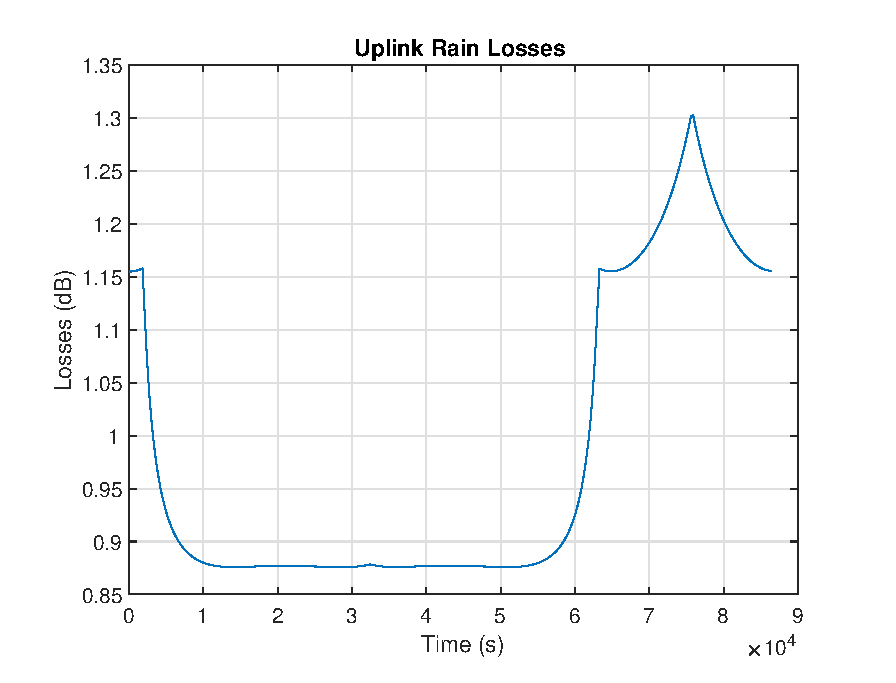
\includegraphics[width = \textwidth]{up_rain.eps}
			\caption{Variation of rain losses in Uplink over the time}
			\label{fig:rain_up}
			\end{minipage}
			\begin{minipage}{.5\textwidth}
			\centering
			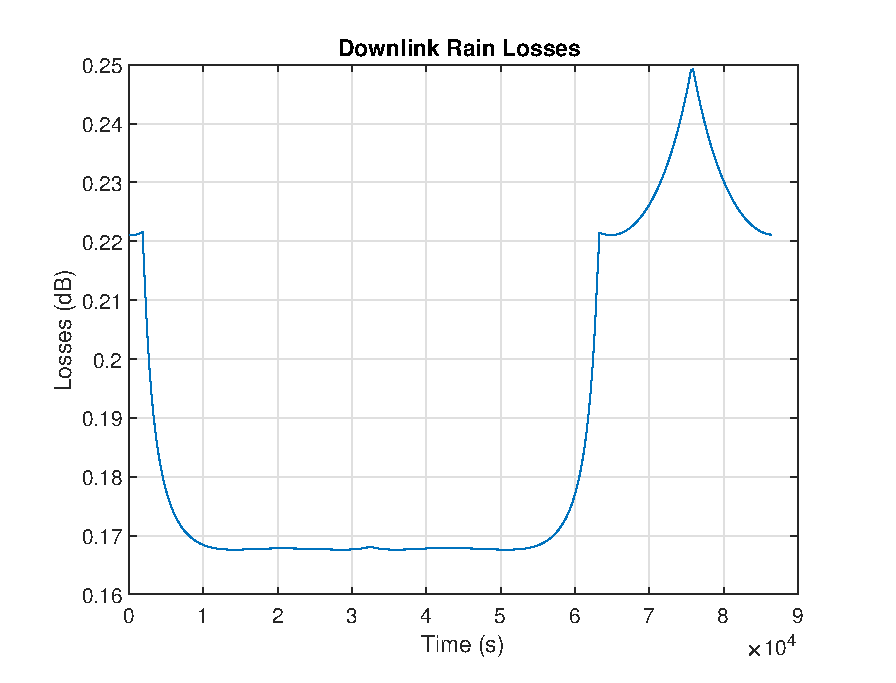
\includegraphics[width = \textwidth]{down_rain.eps}
			\caption{Variation of rain losses in Downlink over the time}
			\label{fig:rain_down}
			\end{minipage}
		\end{figure}

		The parameters in \autoref{eq:rain_formula} are calculated as in \autoref{eq:rain_parameters}.
		\begin{equation}\label{eq:rain_parameters}
			\begin{split}
				k &= 4.21\times 10^{-5}\cdot f^{2.42}\\
				\alpha &= 1.41 \cdot f^{-0-0779}\\
				L_s &= \frac{2km}{sin\theta}\\
				r_p &= \frac{90}{90+4L_scos\theta}
			\end{split}
		\end{equation}
		where $f$ is the carrier frequency in Uplink or in Downlink and $\theta$ is the elevation angle.

		The path loss also depends on the position of the satellite and is calculated with the formula in \autoref{eq:path_loss}, where $r$ is the distance between the satellite and the \gls{gs} or the user, taking in account the altitude of the latter, and $\lambda$ is the wavelength of the communication.

		\begin{equation}\label{eq:path_loss}
			L_{PL} = 20log\bigg(\frac{2\pi r}{\lambda}\bigg) ~dB
		\end{equation}

		Using \autoref{eq:path_loss} in each istant of the simulation, we obtain the plots in \autoref{fig:up_pathloss} and \autoref{fig:down_pathloss}.

		\begin{figure}[ht]
			\begin{minipage}{.5\textwidth}
			\centering
			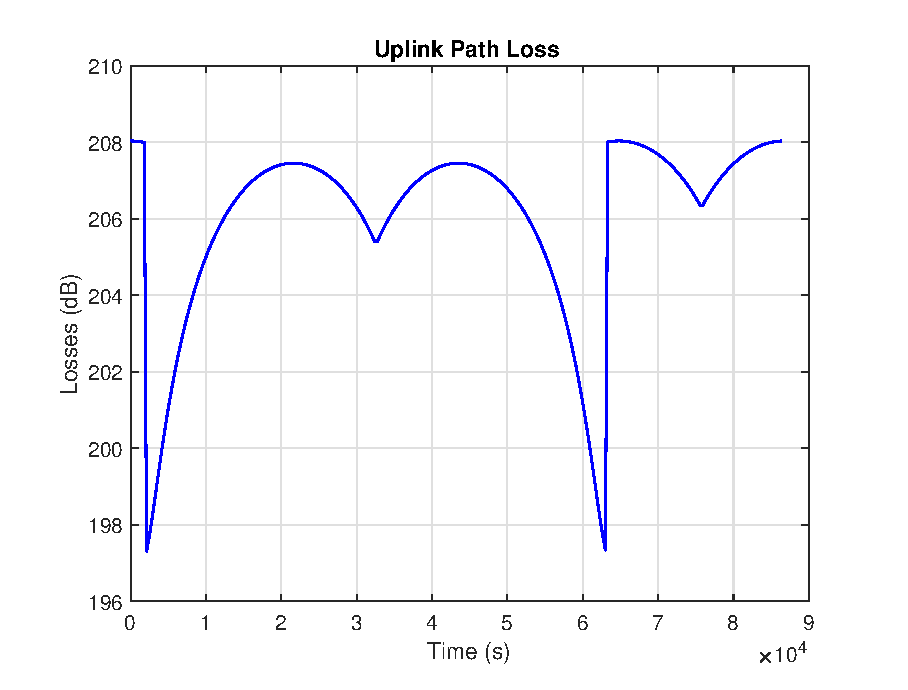
\includegraphics[width = \textwidth]{up_pathloss.eps}
			\caption{Variation of Path Loss in Uplink over the time}
			\label{fig:up_pathloss}
			\end{minipage}
			\begin{minipage}{.5\textwidth}
			\centering
			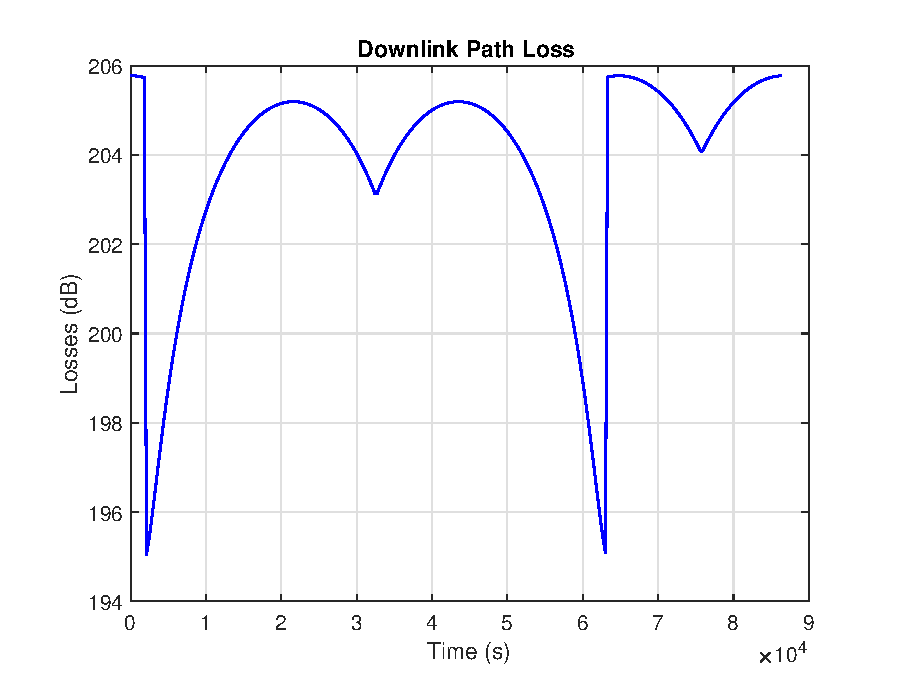
\includegraphics[width = \textwidth]{down_pathloss.eps}
			\caption{Variation of Path Loss in Downlink over the time}
			\label{fig:down_pathloss}
			\end{minipage}
		\end{figure}
	\subsubsection{Effective Isotropic Radiated Power(EIRP)}
	To calculate \gls{eirp} we have to compute firstly the power that each antenna has to transmit $p_{tx}$.
	The power that each transponder has to transmit is calculated as in \autoref{eq:power_1T}, using the parameters yet defined, than this power has to be multiplied for the number of transponder in the system, that in our case is 12, the final formula is in
	\begin{equation}\label{eq:power_1T}
		p_{tx}^{1T} = [p_{HPA}]_{dB} - l_{mc} - l_{ftx}
	\end{equation}
	\begin{equation}\label{eq:power_tot}
		p_{tx} = p_{tx}^{1T} + 10log(12)
	\end{equation}
	Then the \gls{eirp} is calculated for Uplink and Downlink with the formula in \autoref{eq:eirp}.
	\begin{equation}\label{eq:eirp}
		EIRP = G_{tx} + p_{tx}
	\end{equation}
	For the Uplink, using $G_{GS}^{TX}$ as gain, the result is $EIRP_{GS} = 96.79 ~dB$, while for the Downlink, using $G_{SAT}^{TX}$ as gain, the result is $EIRP_{SAT} = 66.58 ~dB$.
\subsection{Uplink}
\subsection{Downlink}
\subsection{Overall Link Budget}


\section{Cost Estimation}
	\subsection{Spacecraft cost}
	The spacecraft cost can be estimated depending on several parameters and criteria, such as the type of mission, the 				subsystem considered and the unit over which calculate the cost. In our specific case we concentrated on the cost analysis 		for a communication-type satellite and review it for every subsystem of the spacecraft and its launch procedure.\\

	The subsystems analyzed  are the following:
	\begin{itemize}
		\item Attitude determination and Control subsystem (ADCS)
		\item Communication subsystem
		\item Electrical power subsystem (EPS)
		\item Integration assembly and test (IA\&T)
		\item Passive sensor
		\item Propulsion
		\item System engineering
		\item Structure
		\item Thermal control
		\item Telemetry tracking and command (TT\&C)
	\end{itemize}
	In particular, \autoref{fig:torta} shows the cost percentage that each system represents: from it we can see that the 				System engineering is the most important item, followed by the EPS and the IA\&T subsystems. Moreover, 						\autoref{fig:distribution} lists the different sections, depending on the type of mission the satellite is intended to 					accomplish, with their standard deviations; tables \ref{fig:mission} and \ref{fig:mission_pound}, instead, show the total 			cost depending on the mission type and the total cost per pound.

	\begin{figure}
		\centering
		\includegraphics[width = .7\textwidth]{Torta.png}
		\caption{Communication spacecraft cost composition}
		\label{fig:torta}
	\end{figure}

	\begin{figure}
		\centering
		\includegraphics[width = 1\textwidth]{Standard_dev.png}
		\caption{Communication spacecraft cost composition: averages and standard deviations}
		\label{fig:distribution}
	\end{figure}

	\begin{figure}
		\centering
		\begin{minipage}{1\textwidth}
		\centering
		\includegraphics[width = .95\textwidth]{Mission.png}
		\caption{Total spacecraft cost}
		\label{fig:mission}
		\end{minipage}
		\hspace{20mm}
		\begin{minipage}{.95\textwidth}
		\centering
		\includegraphics[width = .95\textwidth]{Mission_pound.png}
		\caption{Total spacecraft cost per pound}
		\label{fig:mission_pound}
		\end{minipage}
	\end{figure}

	Regarding the cost per subsystem, \autoref{tab:systems1} and \autoref{tab:systems2} show the different cost each 				subsystem is intended to have:

	\begin{table}
		\centering
		\begin{tabular}{ccc}
		\toprule
		Subsystem & Mean Cost (k\euro) & Standard deviation\\
		\midrule
		IA\&T     & 8311,49   & 8719,94\\
		EPS        & 8441,34   & 5681,80\\
		Structure & 4111,49   & 2955,92\\
		SEPM      & 12167,05 & 7825,63\\
		Thermal  & 903,45    & 562,3\\
		TT\&C    & 4423,24   & 2942,24\\
		\bottomrule
		\end{tabular}
		\caption{List of the costs per subsystem}
		\label{tab:systems1}
	\end{table}

	\begin{table}
		\centering
		\begin{tabular}{ccc}
		\toprule
		Subsystem & Mean Cost/unit (k\euro/kg or ch) & Standard deviation\\
		\midrule
		ADCS                                         & 94,70     & 8719,94\\
		Communication ($1 < ch < 10$)   & 3923,19 & 1443,98\\
		Communication ($10 < ch < 25$) & 1534,45 & 558,37\\
		Communication ($25 < ch$)         & 708,40   & 197,35\\
		EPS                                            & 24,7      & 7,27\\
		Propulsion                                  & 54,68     & 14,32\\
		Structure                                    & 15,94     & 4,37\\
		\bottomrule
		\end{tabular}
		\caption{List of the costs per subsystem per pound/channel}
		\label{tab:systems2}
	\end{table}

	Through this data we can make a raw hypothesis on the average total cost of the spacecraft with a summary estimation 			of its mass:

	\begin{table}
		\centering
		\begin{tabular}{ccc}
		\toprule
		\multicolumn{3}{c}{Communication spacecraft}\\
		\midrule
		IA\&T       & 8311,49 \euro       & $+$\\
		EPS          & 24,7 \euro/Kg        & $\times NCHILI +$\\
		Structure   & 15,94  \euro/Kg     & $\times NCHILI +$\\
		SEPM        & 12167,05 \euro     & $+$\\
		Thermal    & 903,45 \euro        & $+$\\
		TT\&C       & 4423,24 \euro      & $+$\\
		ADCS        & 94,70 \euro/Kg     & $\times NCHILI +$\\
		Propulsion & 54,68   \euro/Kg   & $\times NCHILI +$\\
		Communication ($10 < ch < 25$) & 1534,45 \euro/ch & $\times 12 ch =$\\
		\bottomrule
		Total cost:& & TOT\\
		\end{tabular}
		\caption{List of the costs per subsystem per pound/channel}
		\label{tab:cost}
	\end{table}
\subsection{Launch cost}
For the launch cost we based our considerations on the prices listed by the $SpaceX$ company. \autoref{fig:spacex} shows the prices for different types of launches, depending on the mass of the spacecrafts and the orbits they should reach.

Through the considerations we have made in the previous sections we can state that around $180$ Millions of dollars ($151.793.055$ \euro \cri{verifica il prezzo}) are needed for the launch: in fact each spacecraft has a total mass of about \cri{mettere massa} and the Molniya orbit is a HEO orbit; moreover, since the raans of the two orbital planes are separated of 180 $\deg$ it is necessary to use two separate launchers, one for each spacecraft.\\

Through this analysis the total cost for the project is:
\begin{equation}
Cost_{Total} = Cost_{Launch} + Cost_{Spacecraft} = \cri{Mettere costo finale} \text{\euro}
\end{equation}

\begin{figure}
\centering
\includegraphics[width = .9\textwidth]{Spacex.png}
\caption{$SpaceX$ price list}
\label{fig:spacex}
\end{figure}


Through the considerations we have made in the previous sections we can state that around $180$ Millions of dollars ($151.793.055$ \euro \cri{verifica il prezzo}) are needed for the launch: in fact each spacecraft has a total mass of about \cri{mettere massa} and the Molniya orbit is a HEO orbit; moreover, since the raans of the two orbital planes are separated of 180 $\deg$ it is necessary to use two separate launchers, one for each spacecraft.\\

Through this analysis the total cost for the project is:
\begin{equation}
Cost_{Total} = Cost_{Launch} + Cost_{Spacecraft} = \cri{Mettere costo finale} \text{\euro}
\end{equation}

\begin{figure}
\centering
\includegraphics[width = .9\textwidth]{Spacex.png}
\caption{$SpaceX$ price list}
\label{fig:spacex}
\end{figure}

\section{Final considerations and conclusions}
	With this work we intended to present a communication system aimed to service the polar regions over Europe and Russia. From the previous sections the values and parameters found permitted us to establish the reliability and the feasibility of our system in terms of cost and weight. From our calculations we obtained a relatively simple system which needs 2 satellites and one ground station to supply our purpose and guarantees continuous coverage of the interested zones, moreover the link budget analysis provides us satisfactory values for the communication link, at the same time requiring a not so power-costly technology (see the modulation choice or the power for the \gls{hpa} based on worst case analysis). Finally, the cost analysis outlines a project which could represent a typical market solution, even though the one presented here is just a first proposal and it could be refined with more time and a comparison to other approaches.

\bibliographystyle{IEEEtran}
\bibliography{IEEEabrv,bibliography}

\end{document}
